\section{Problem Demonstration}
\label{sec:motiv}
%\begin{figure}[t!]
%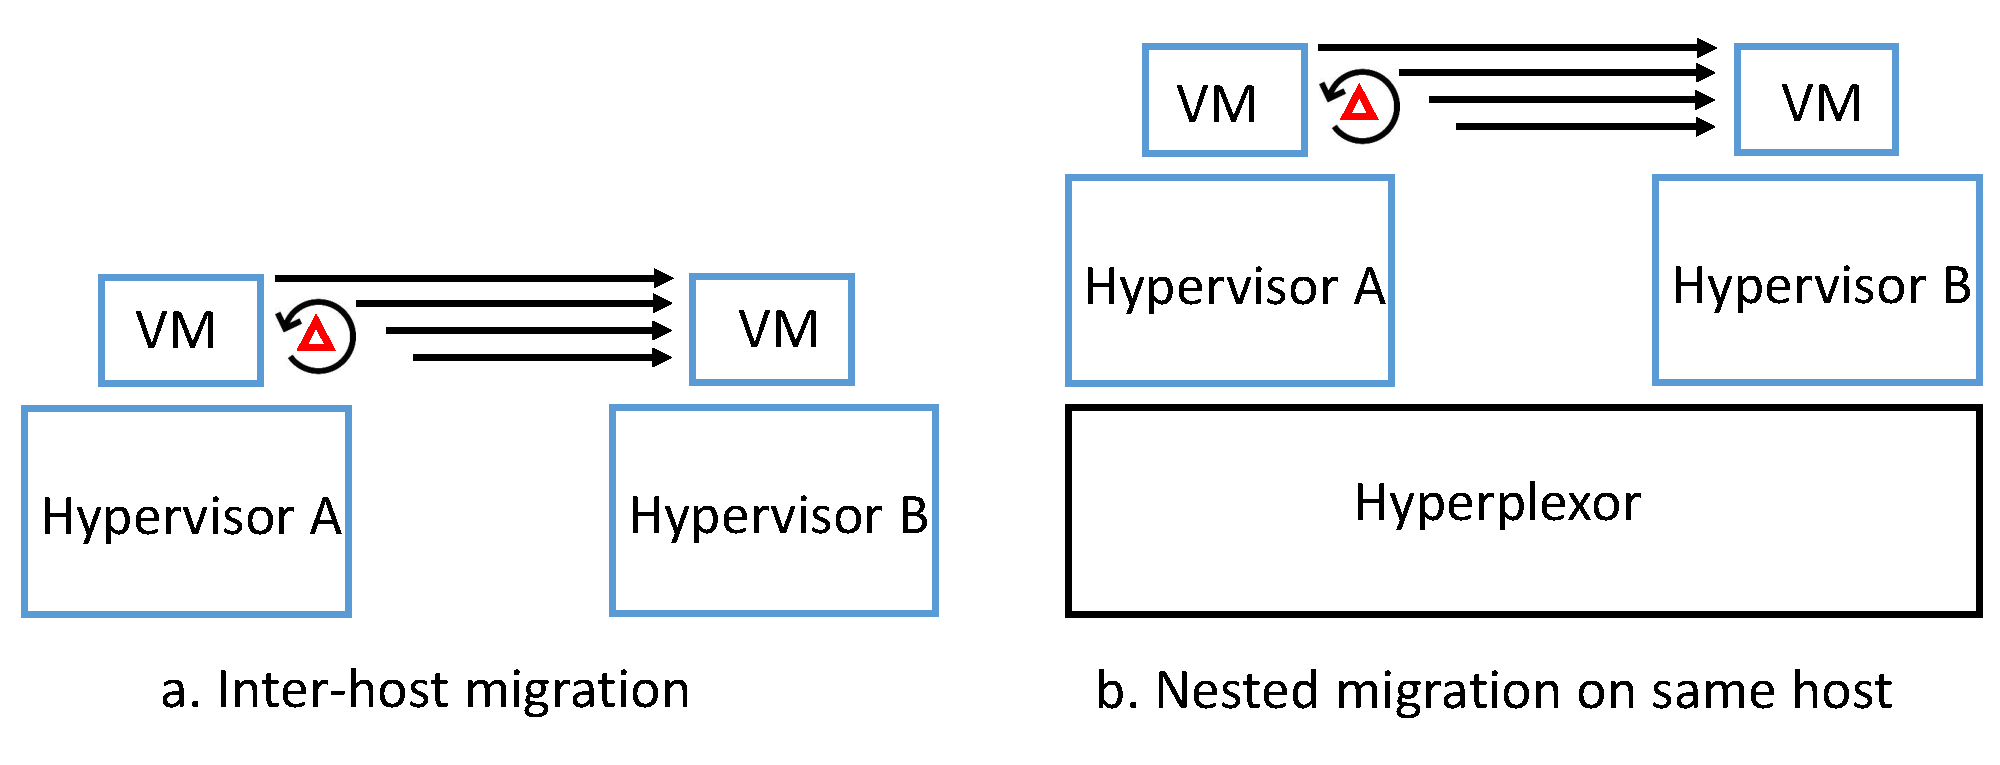
\includegraphics[width=0.45\textwidth]{figures/pre-copy-with-subtitles.pdf}
%\caption{Replacing hypervisor using a. Inter-host migration b. Nested migration on same host}
%\label{fig:motivsetup}
%\end{figure}
In this section, we examine the performance of traditional live migration for hypervisor replacement 
to motivate the need for a faster remapping-based mechanism.

\begin{figure} 
	\centering
	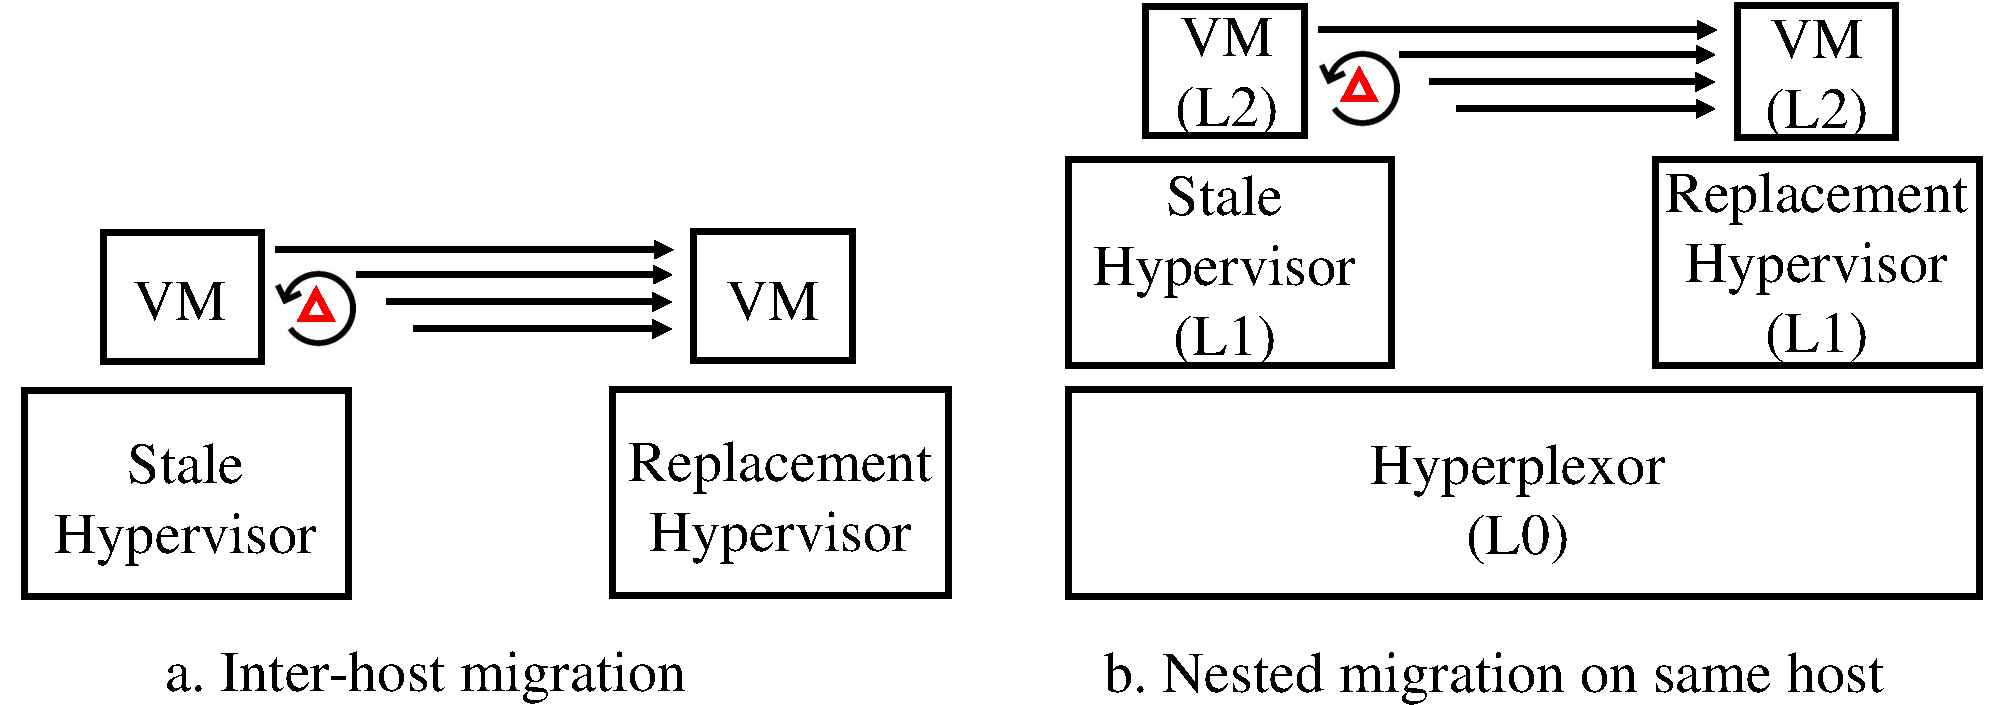
\includegraphics[width=0.45\textwidth]{figures/setups.pdf}
	\caption{Replacing hypervisor in (a) Inter-host setup (b) Nested setup.}
	\label{fig:motivsetup}
\end{figure}

\subsection{Using pre-copy for hypervisor replacement}
%\begin{itemize}[leftmargin=0.15 in]
\para{Inter-Host Live VM Migration:} To refresh a hypervisor, a traditional approach is to live 
migrate VMs from their current host to another host (or hosts) having an updated hypervisor. 
As shown in Figure \ref{fig:motivsetup}a, we can leverage the  state-of-the-art pre-copy live 
VM migration technique. Pre-copy VM live migration consists of three major phases: iterative 
memory pre-copy rounds, stop-and-copy, and resumption.
During the memory pre-copy phase, the first iteration transfers all 
memory pages over the network to the destination, while the VM continues to execute concurrently. 
In the subsequent iterations, only the dirtied pages are transferred. 
After a certain round of iterations, determined by a convergence criteria, the stop-and-copy phase
is initiated, during which the VM is paused at the source and any remaining dirty pages, VCPUs, 
and I/O state are transferred to the destination VM. Finally, the VM is resumed at the destination.

\para{Intra-Host Live VM Migration:} As shown in Figure \ref{fig:motivsetup}b, using nested virtualization, a base hyperplexor at layer-0 (L0) can run deprivileged hypervisors at layer-1 (L1), which control the VMs running at layer-2 (L2). At hypervisor replacement time, the hyperplexor can boot a new replacement hypervisor at L1, and use intra-host live VM migration to transfer VMs from the stale hypervisor to the replacement hypervisor.
%\end{itemize}

%with The objective of HyperFresh is to replace hypervisor beneath the guest with minimal service disruption and performance degradation in guests. The parameters that affect the performance of applications running in the guest are total migration time and downtime. The time from initialization phase to the time when the VM resumes at the destination is the total migration time. Downtime is the time during which the VM remains unresponsive.
%We observed that, live migration of 1GB idle guest using default QEMU's pre-copy takes 12s of total migration time over a 20 Gbps network card. The total migration time is high as QEMU limits the default migration bandwidth to 256Mbps. To compare our results with the best case of QEMU, we modified the pre-copy live migration algorithm. 

\begin{figure*}[h!]
	\centering
	\subfloat[Idle guest]{
		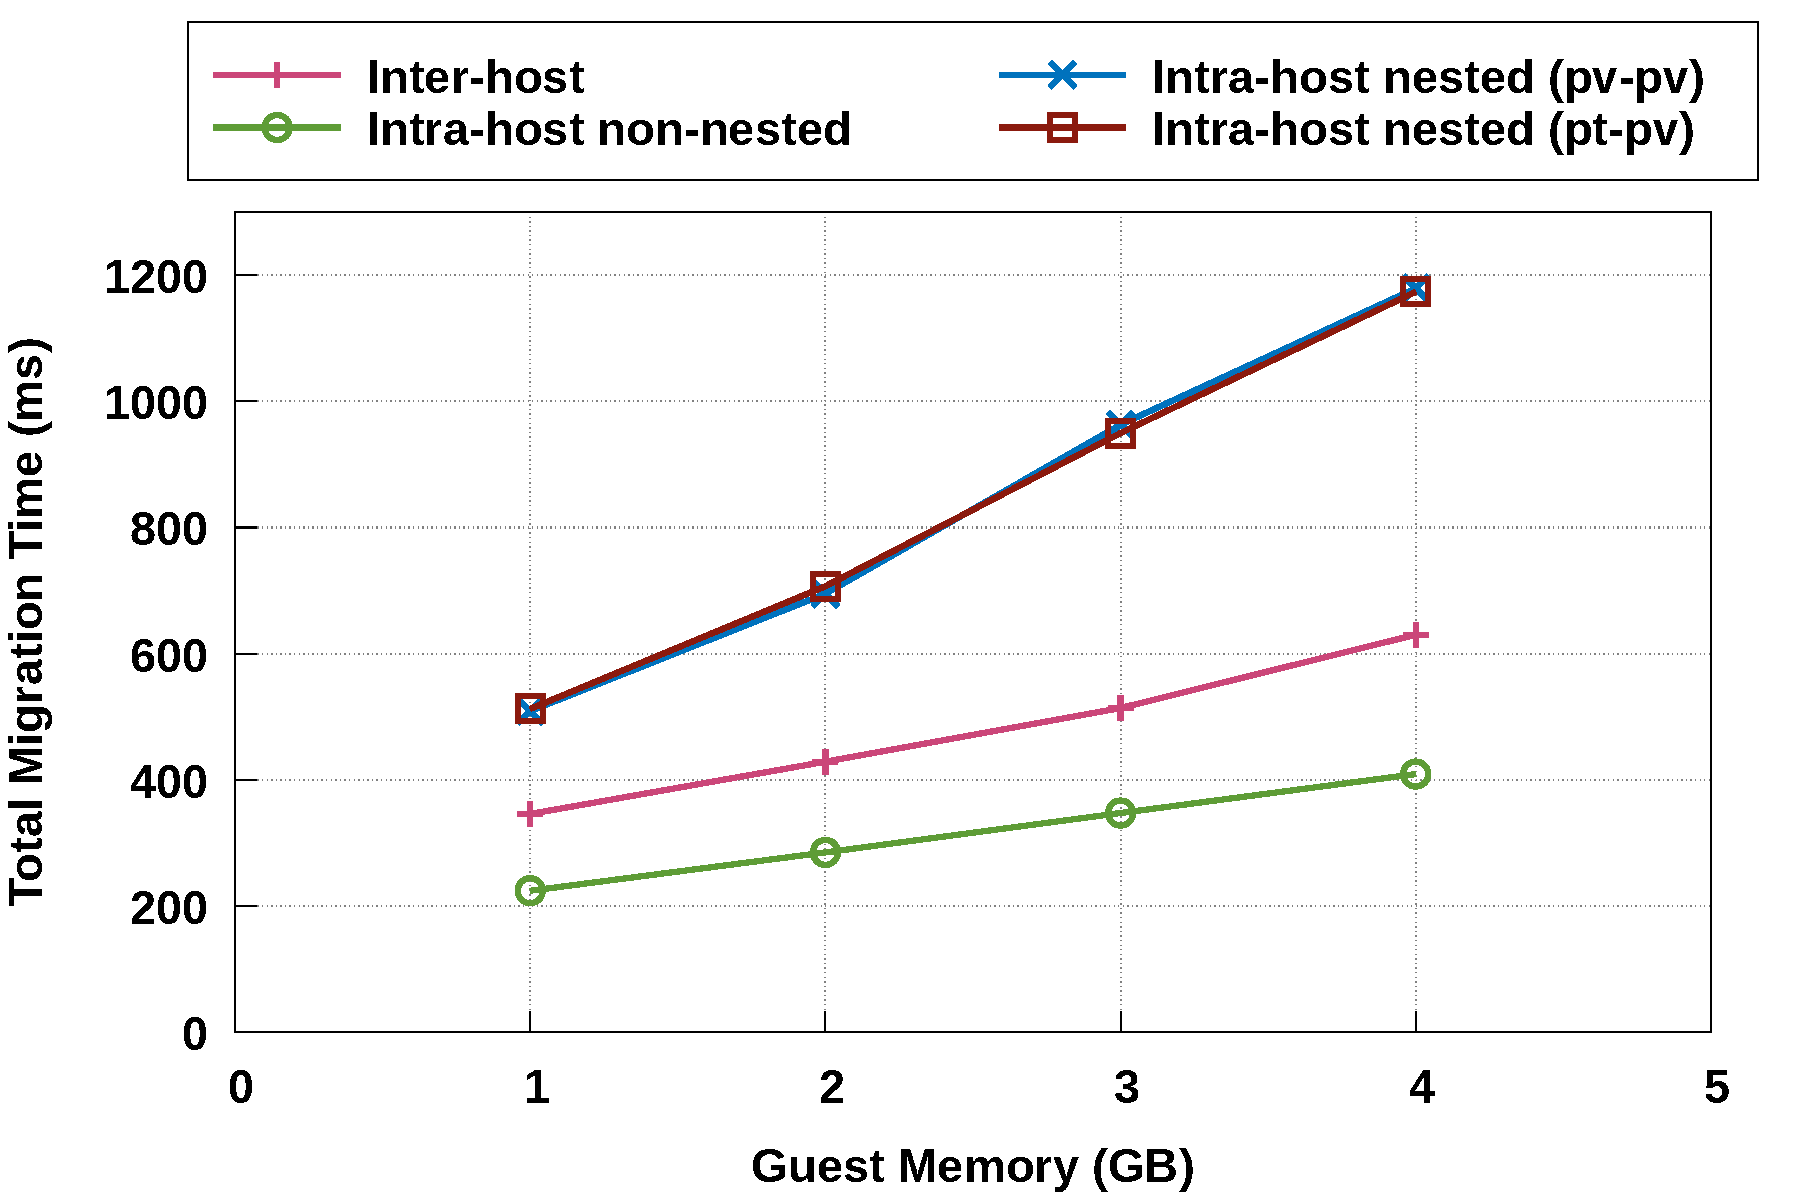
\includegraphics[width=0.48\textwidth]{figures/idle_guest_migration.pdf}}
	\subfloat[Busy guest]{
		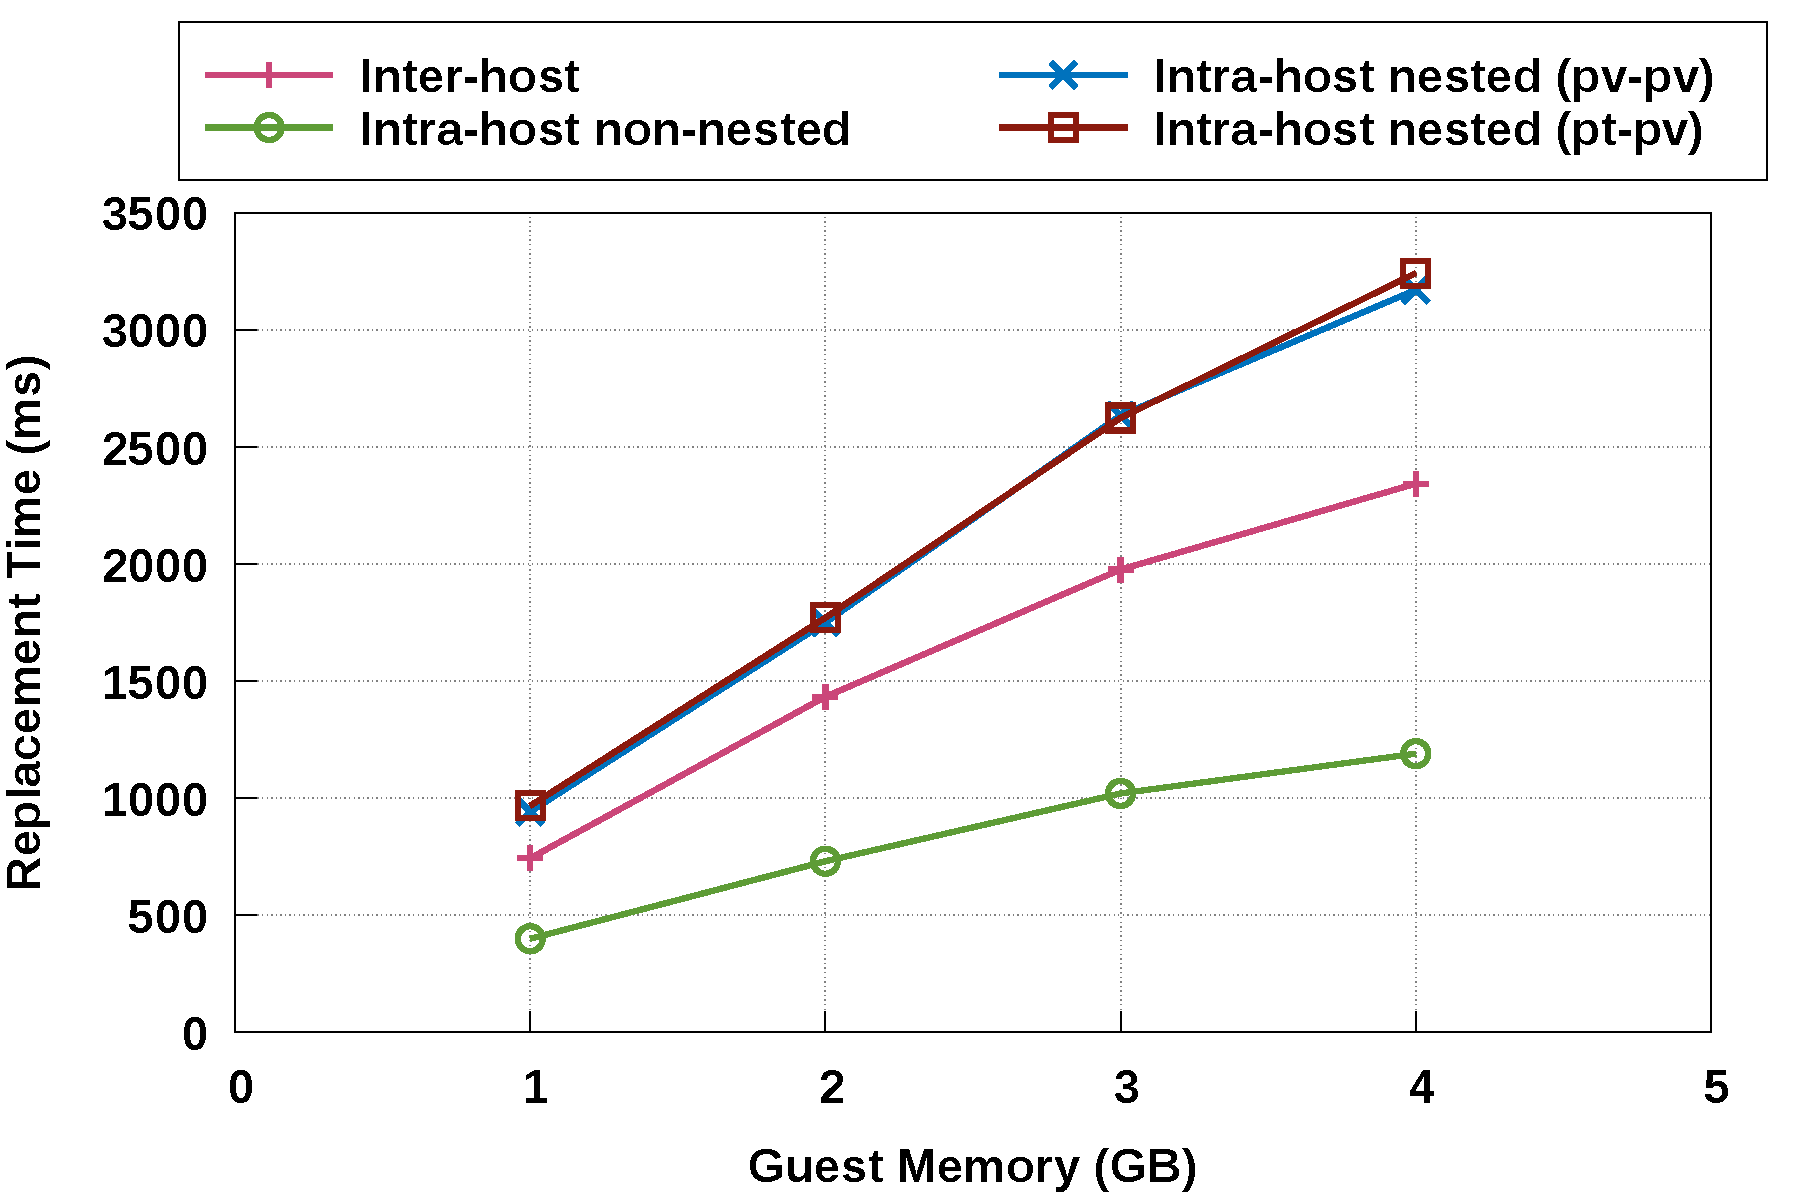
\includegraphics[width=0.48\textwidth]{figures/busy_guest_migration.pdf}}
	\caption{Comparison of hypervisor replacement time between the same and different hosts with nested and non-nested setups.}
	\label{fig:motiv}
\end{figure*}

\subsection{Improving the default pre-copy implementation in KVM/QEMU} 
We observed two performance problems when using the default pre-copy implementation of KVM/QEMU.
So that we can compare our remapping approach with the best case performance of pre-copy implementation, 
we modified the pre-copy implementation as described below. 

First, we observed that the total live migration time for a 1 GB idle VM between two
physical machines connected via a 40 Gbps 
network link was 12 seconds, which was way more than what we expected. 
Upon investigation, we found that, by default, QEMU limits the migration bandwidth to 256 Mbps. 
We modified QEMU to disable this rate limiting mechanism, 
so that the VM's memory can be transferred at full network bandwidth.

Secondly, we observed that when the VM is running a write-intensive workload
then the pre-copy iterations never converge to the stop-and-copy phase.
This was found to be due to an inaccurate convergence criteria
based on the VM's page dirtying rate (the rate at which a VM writes to its memory pages), 
which not only breaks down for write-intensive VMs, 
but also misses opportunities for initiating an earlier stop-and-copy phase 
when the number of dirtied pages in the the last iteration could be low. 

To ensure that the pre-copy rounds converge successfully, we made two additional changes
to QEMU's pre-copy implementation. We placed a hard limit of 20 rounds on the 
maximum number of pre-copy iterations, after which the stop-and-copy phase is initiated.
We also simplified QEMU's default convergence criteria by triggering the
stop-and-copy phase when the number of dirty pages from the prior round is less than 5,000 pages.
The latter change yields a low downtime of less than 5 ms.
%TODO: Kartik: Confirm that the downtime was 5ms.
\footnote{We note that these modifications are meant specifically to improve pre-copy performance in 
our experiments and are not general recommendations for production settings}.


%In addition, to control the downtime and the total migration time for write-intensive workloads, we add the following conditions to move to the {\em stop-and-copy} phase if one of the following conditions is met: (1) The number of dirty pages to be transferred is less than 5000; or (2) If the number of pre-copy iterations exceeds 20. 

%The first condition ensures minimum downtime as the number of pages transferred during last phase is very less. If the workload in the VM is write-intensive, and the rate at which the workload is dirtying the pages is greater than the migration link bandwidth, the migration never converges. To ensure that the migration completes successfully, we restrict the number of pre-copy iterations to 20. After 20 iterations the VM moves to stop and copy phase.

%Guest Memory (GB)	Inter-host	Intrahost non-nested	Intrahost nested (pv-pv)	Intrahost nested (pv-pt)
%1	346.2	224.4	509.2	512.6
%2	429	    285.2	695	    707
%3	514	    347.6	963	    949.6
%4	630.2	409.4	1179	1173.6

%\begin{figure}[t!]
%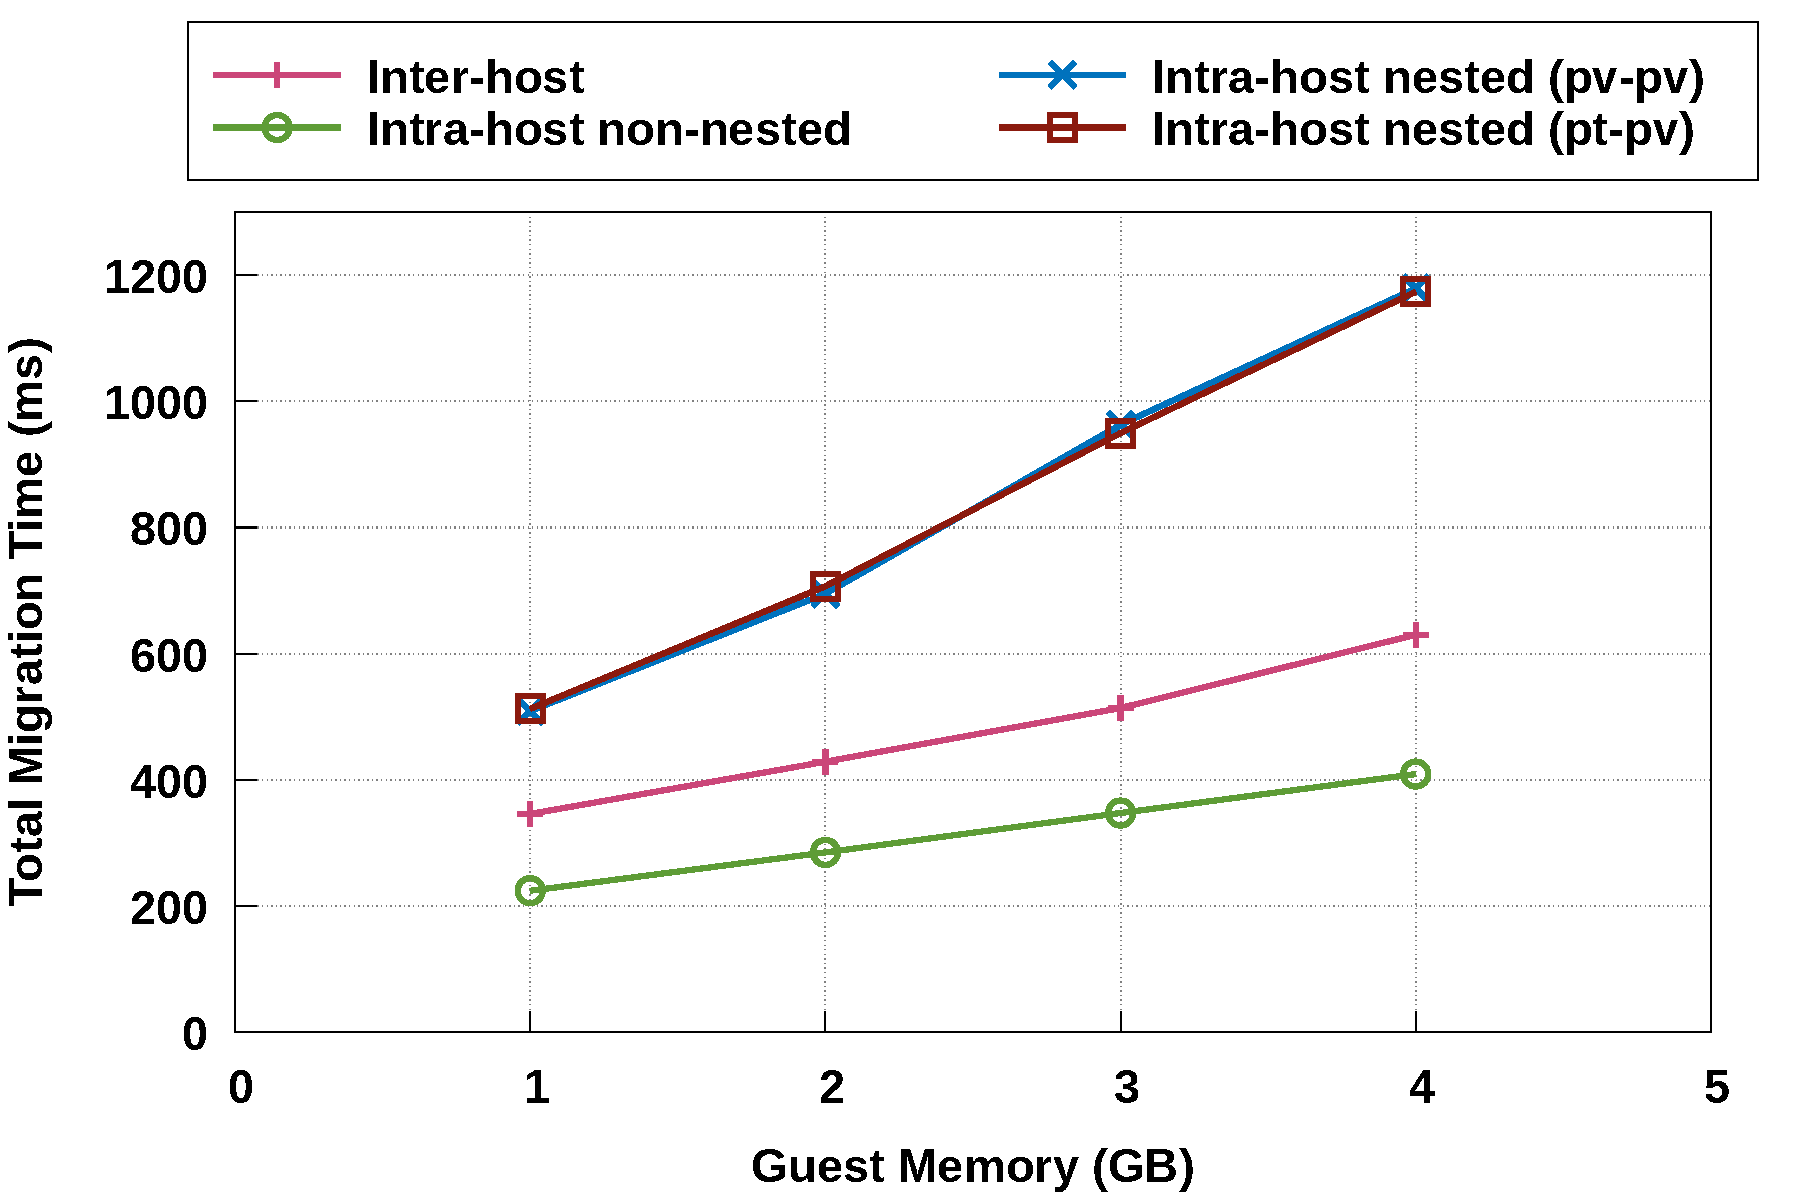
\includegraphics[width=0.45\textwidth]{figures/idle_guest_migration.pdf}
%\caption{Idle guest: Comparison of hypervisor replacement time between the same and different hosts with nested and non-nested setup.}
%\label{fig:motivid}
%\end{figure}

%Guest Memory (GB)	Inter-host	Intrahost non-nested	Intrahost nested (pv-pv)	Intrahost nested (pv-pt)
%1	743.6	399.6	942.4	967.4
%2	1433	730.6	1750	1770.6
%3	1975.8	1020	2634	2623.2
%4	2342.6	1190	3170	3241.6

%\begin{figure}[t!]
%  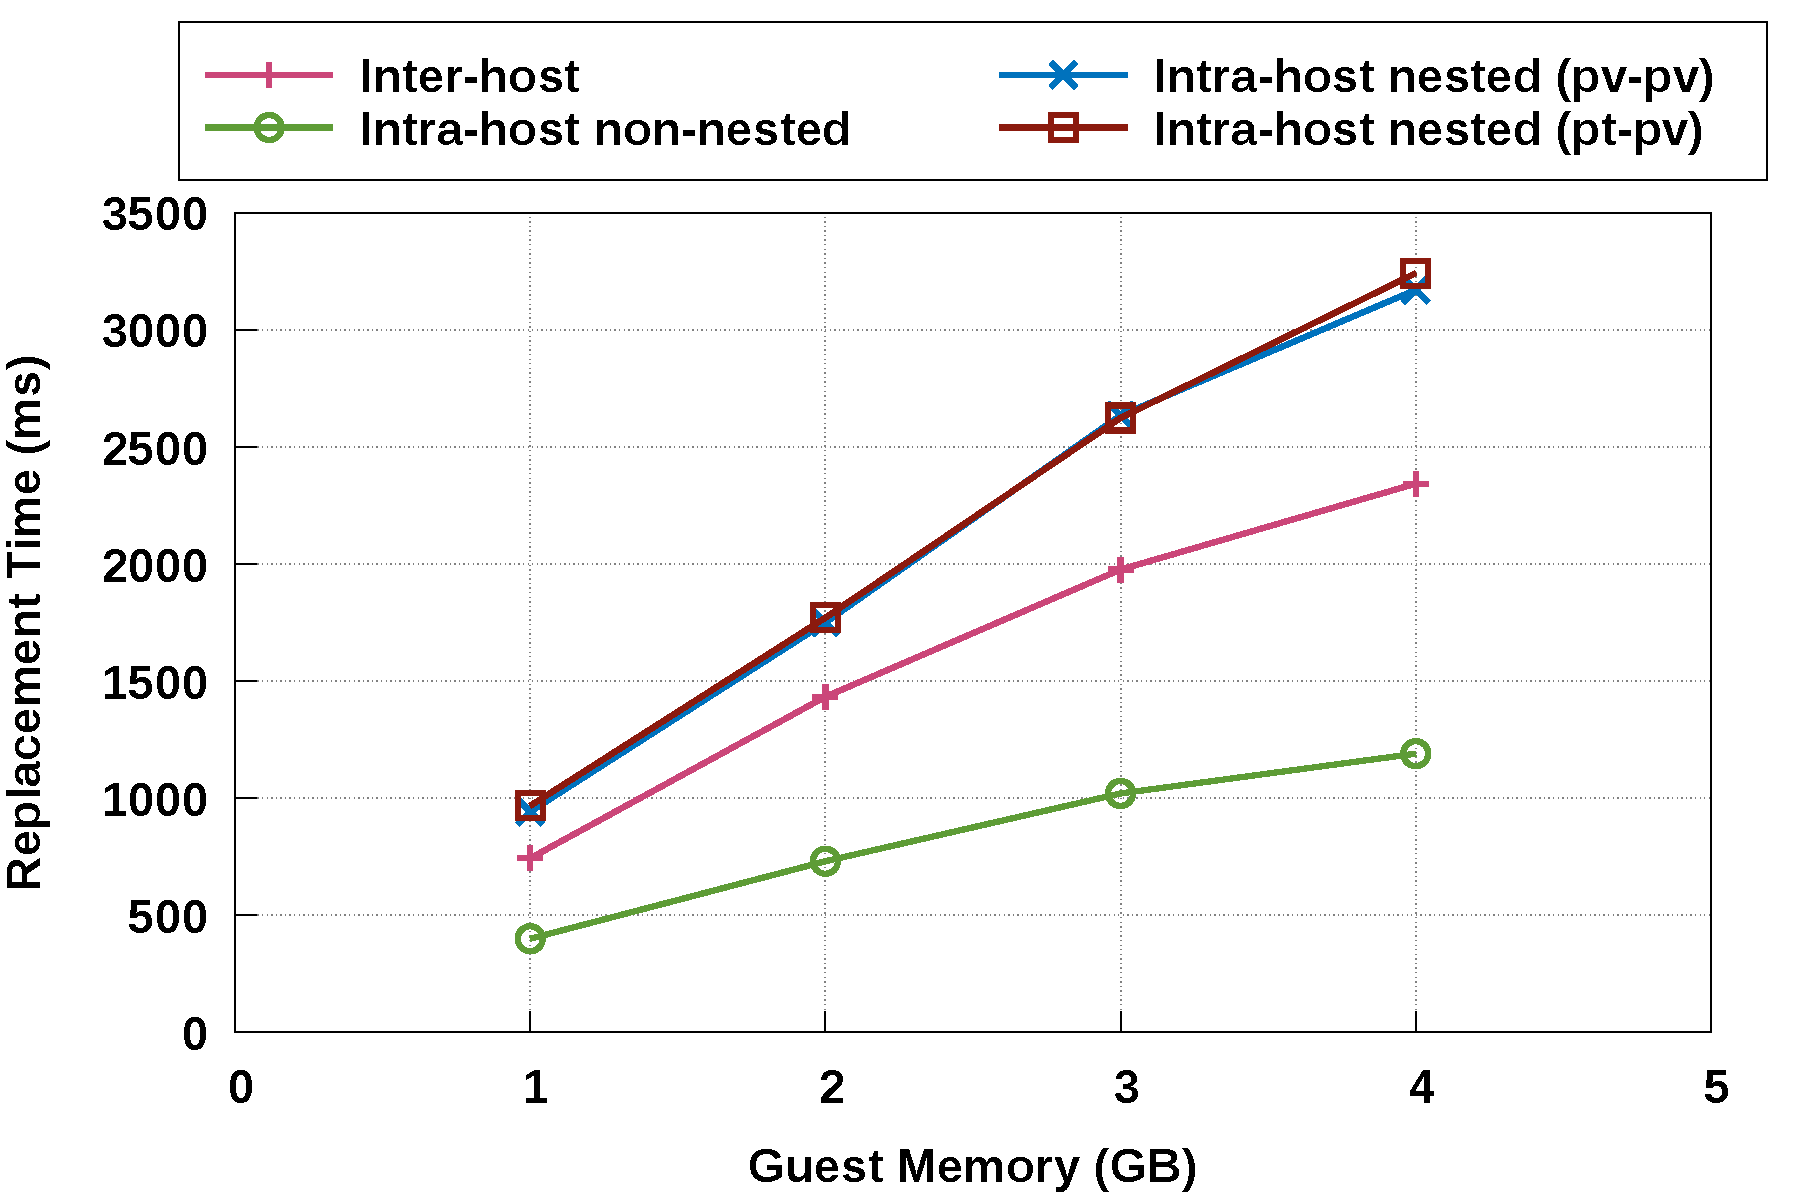
\includegraphics[width=0.45\textwidth]{figures/busy_guest_migration.pdf}
%  \caption{Busy guest: Comparison of hypervisor replacement time between the same and different hosts with nested and non-nested setup.}
%  \label{fig:motivbz}
%\end{figure}

%\begin{figure}
%	\centering
%	\subfloat[Idle guest]{
%		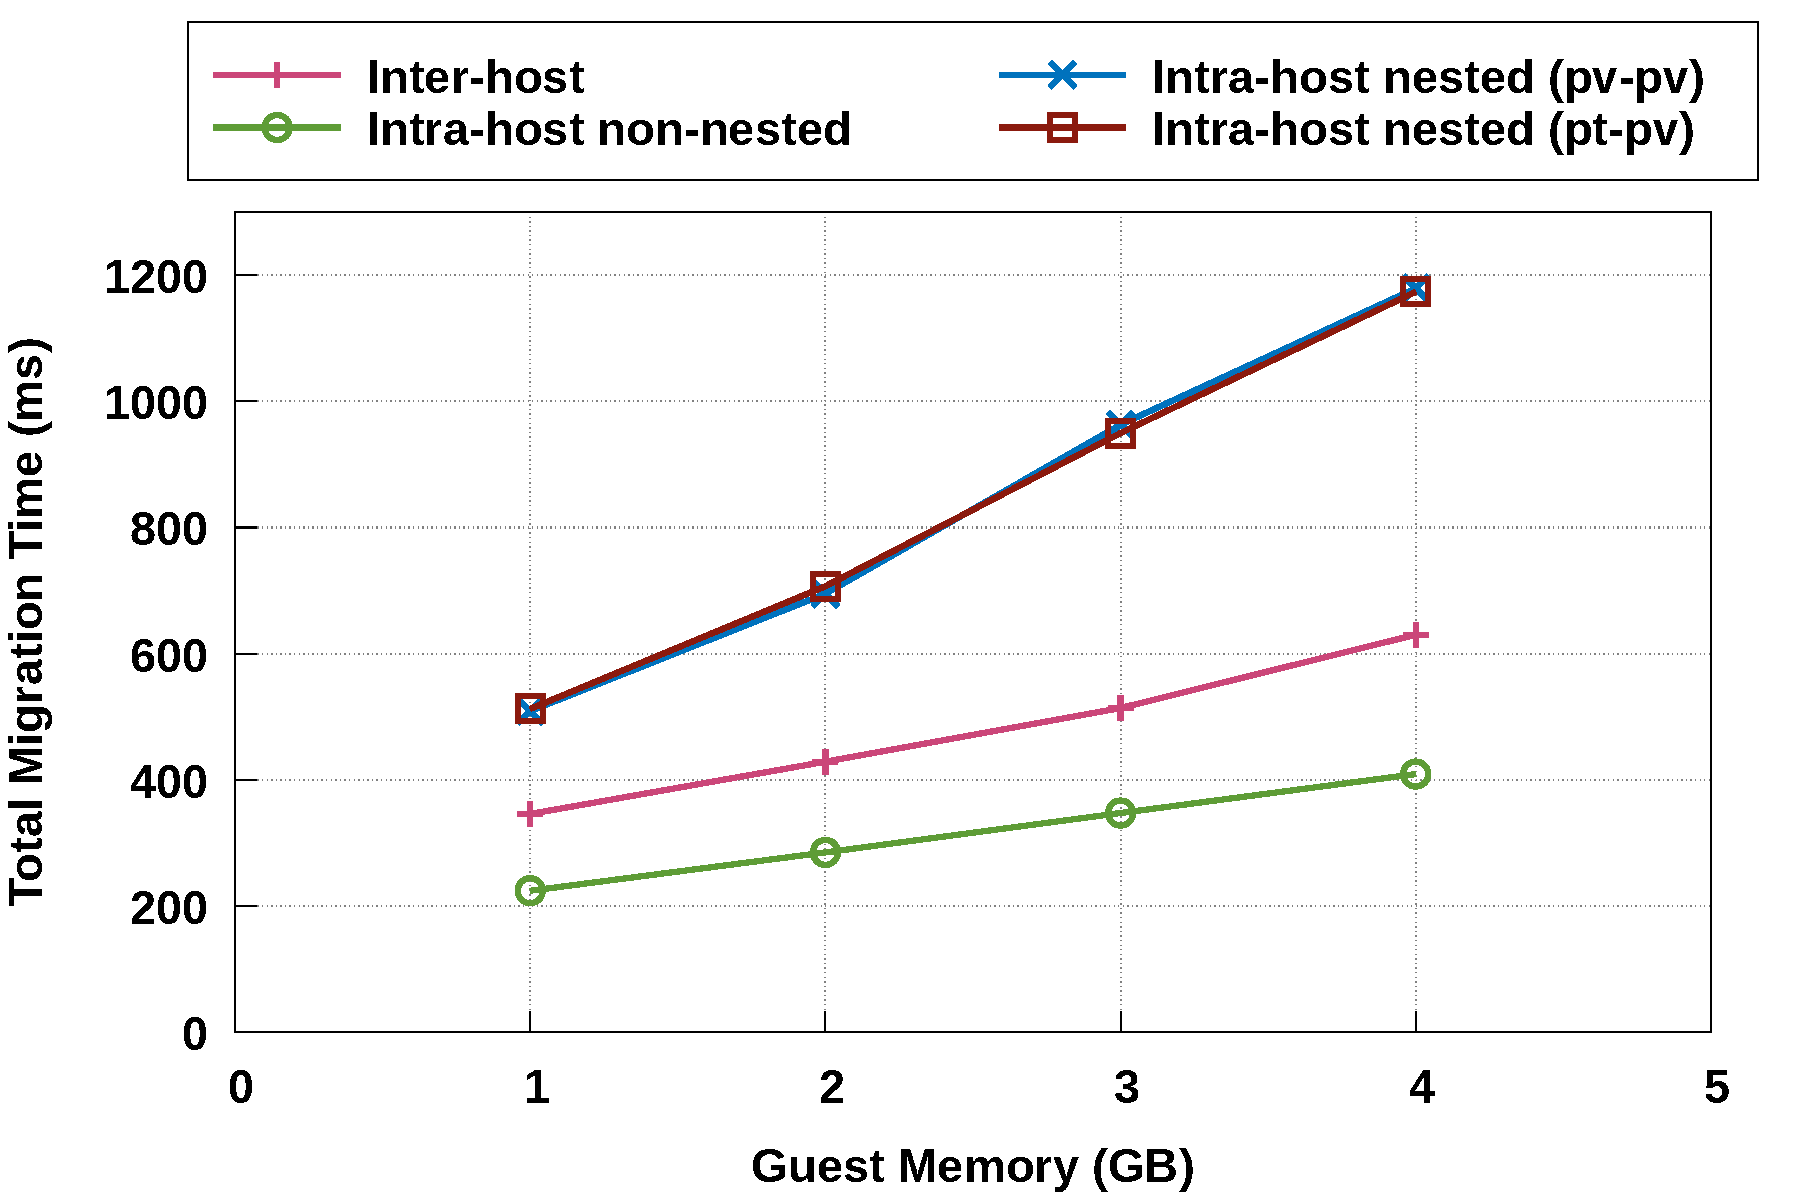
\includegraphics[width=.235\textwidth]{figures/idle_guest_migration.pdf}}
%	\subfloat[Busy guest]{
%		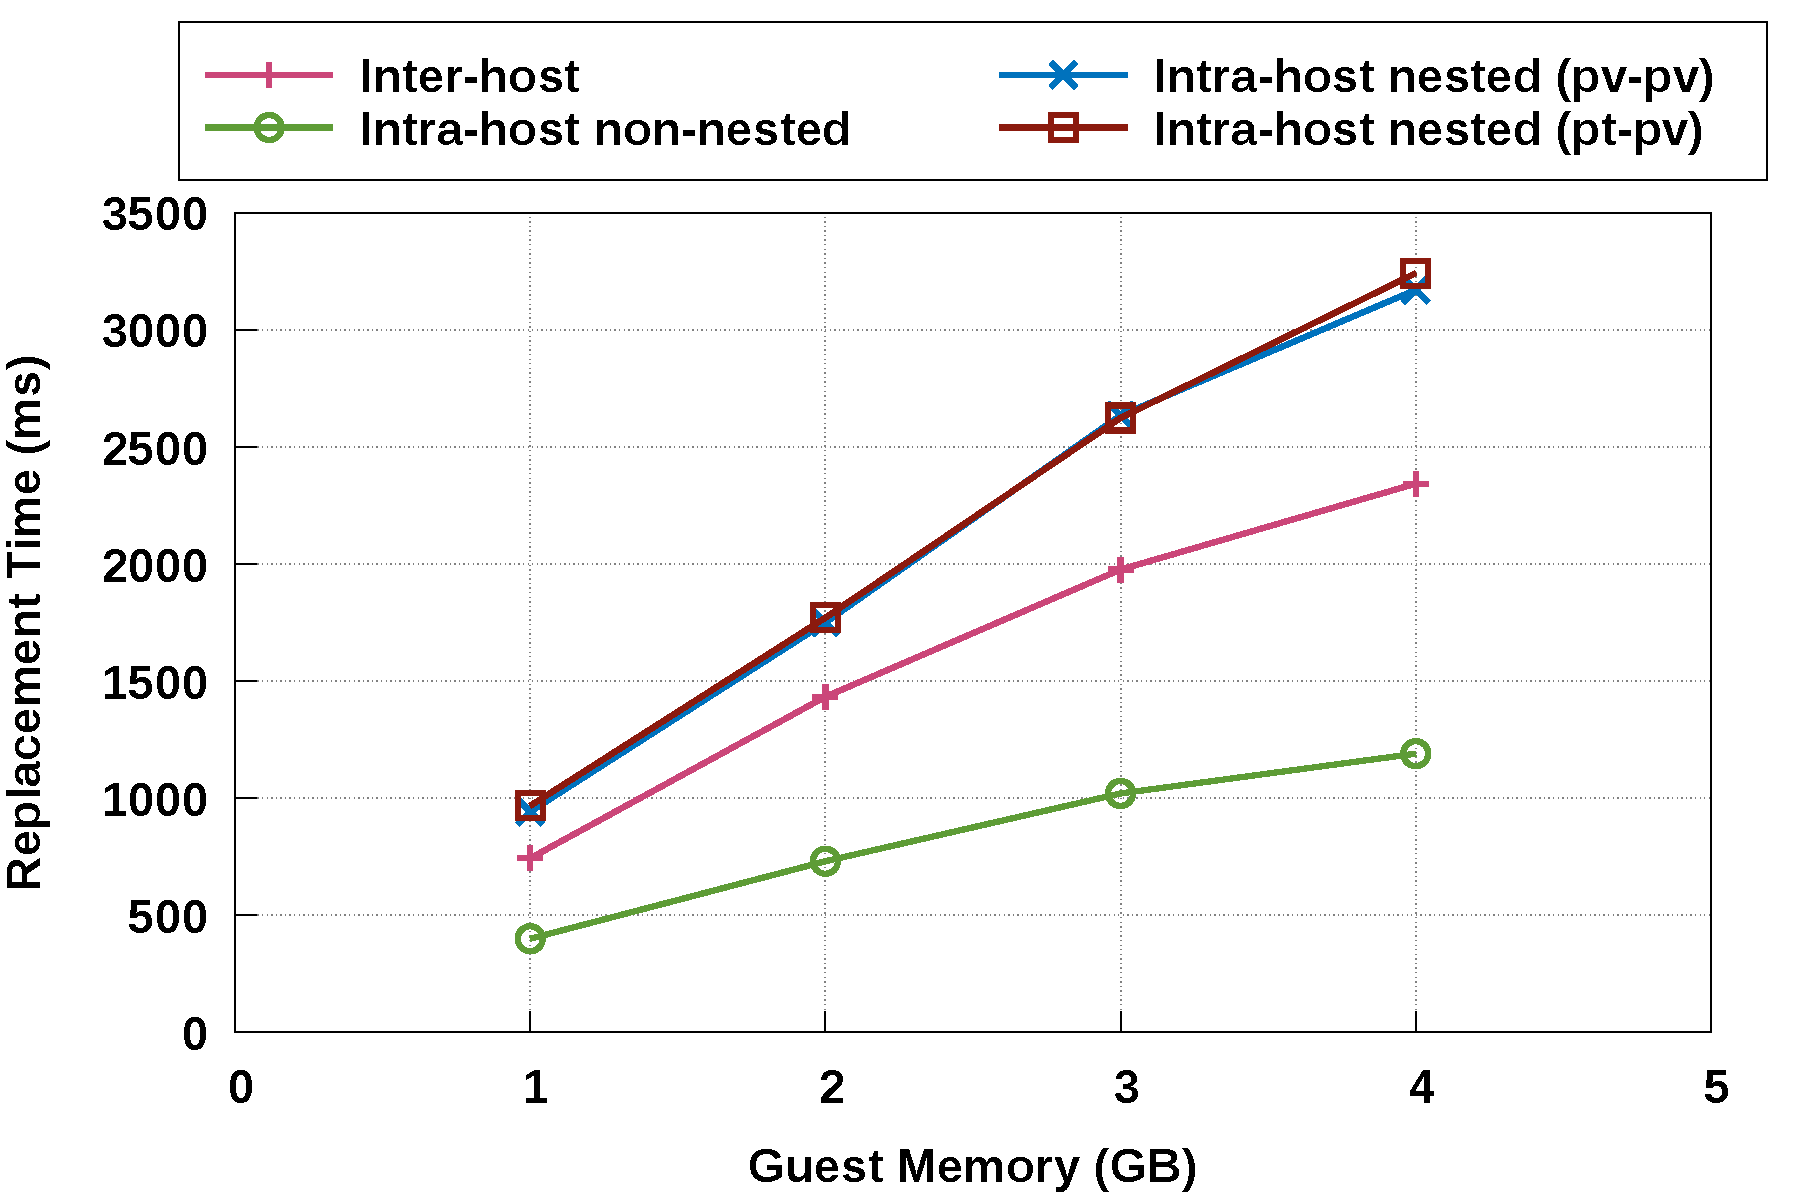
\includegraphics[width=.235\textwidth]{figures/busy_guest_migration.pdf}}
%	\caption{Comparison of hypervisor replacement time between the same and different hosts with nested and non-nested setup}
%	\label{fig:motivid}
%\end{figure}

%\begin{figure}
%	\centering
%	\subfloat[Idle guest]{
%		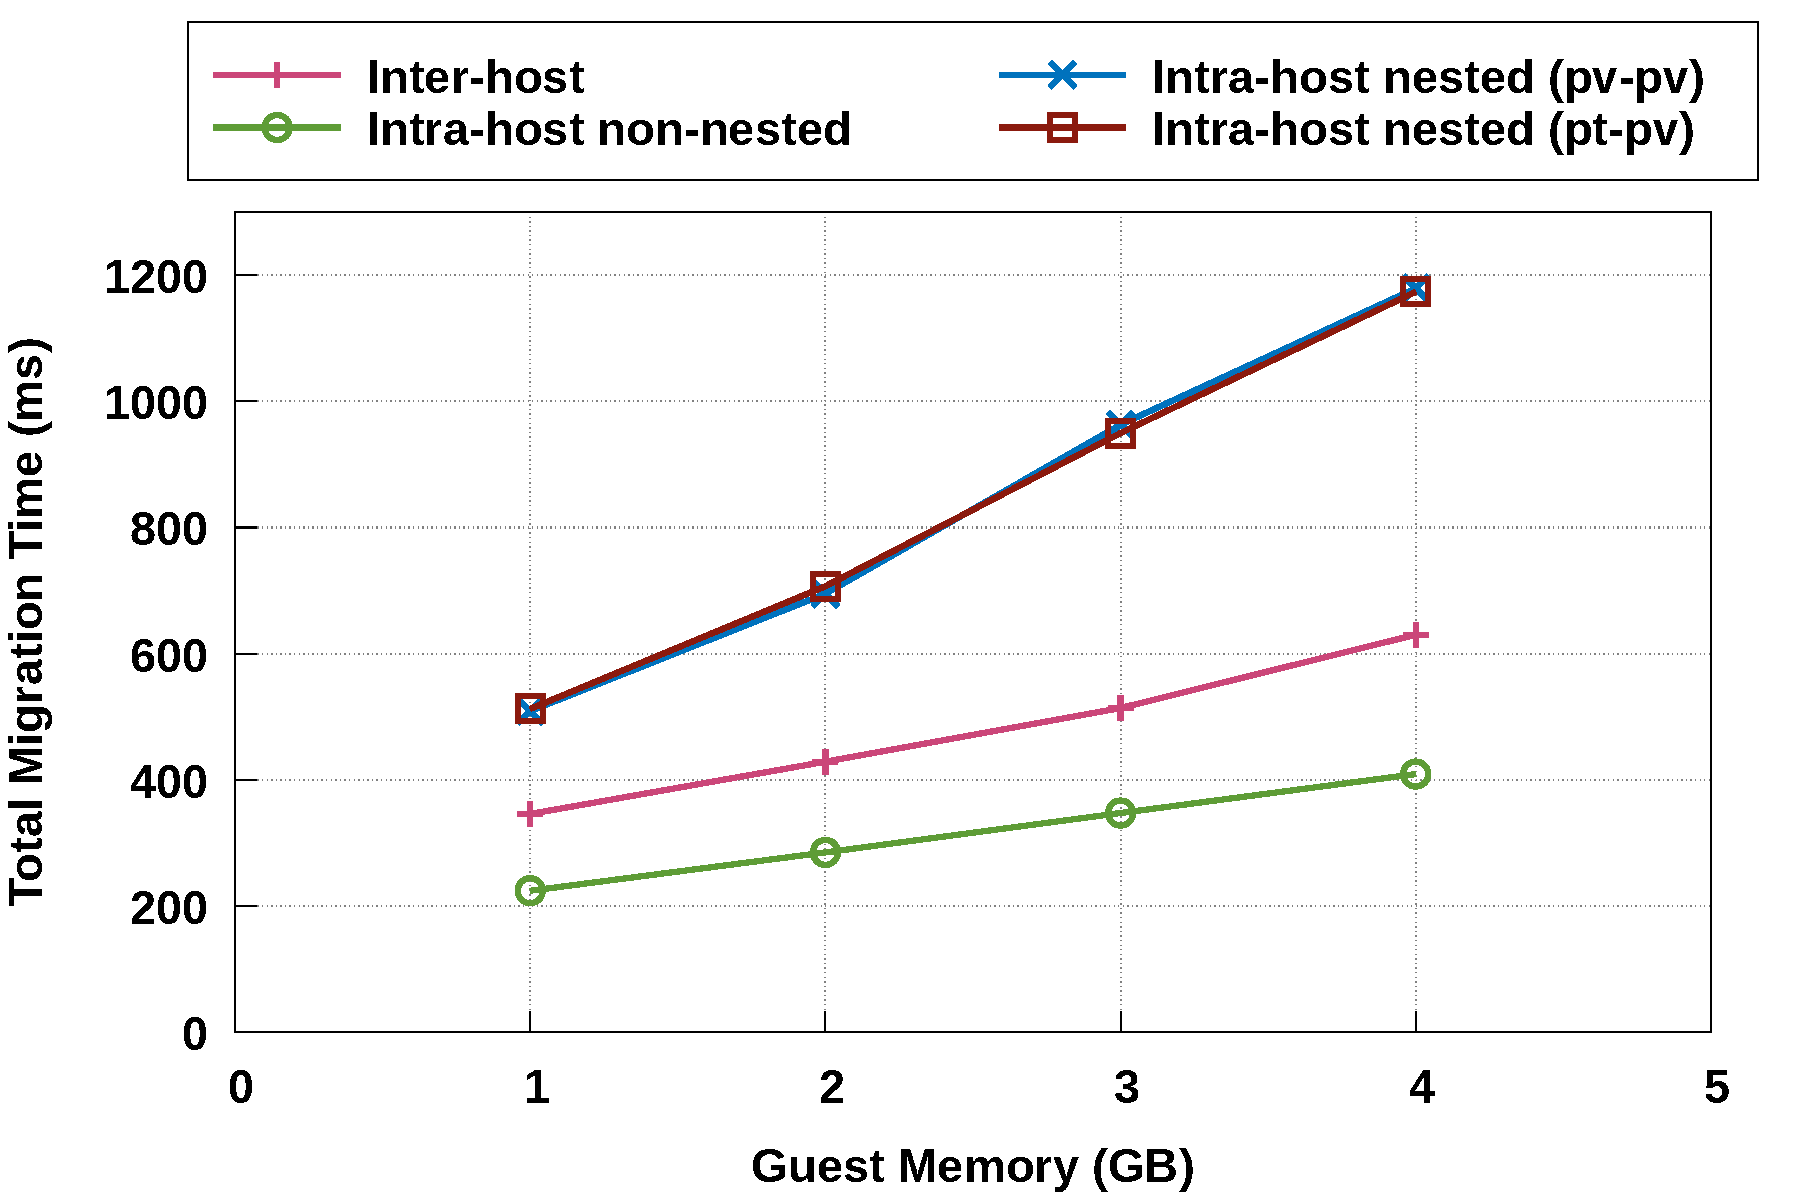
\includegraphics[width=.235\textwidth]{figures/idle_guest_migration.pdf}}
%	\subfloat[Busy guest]{
%		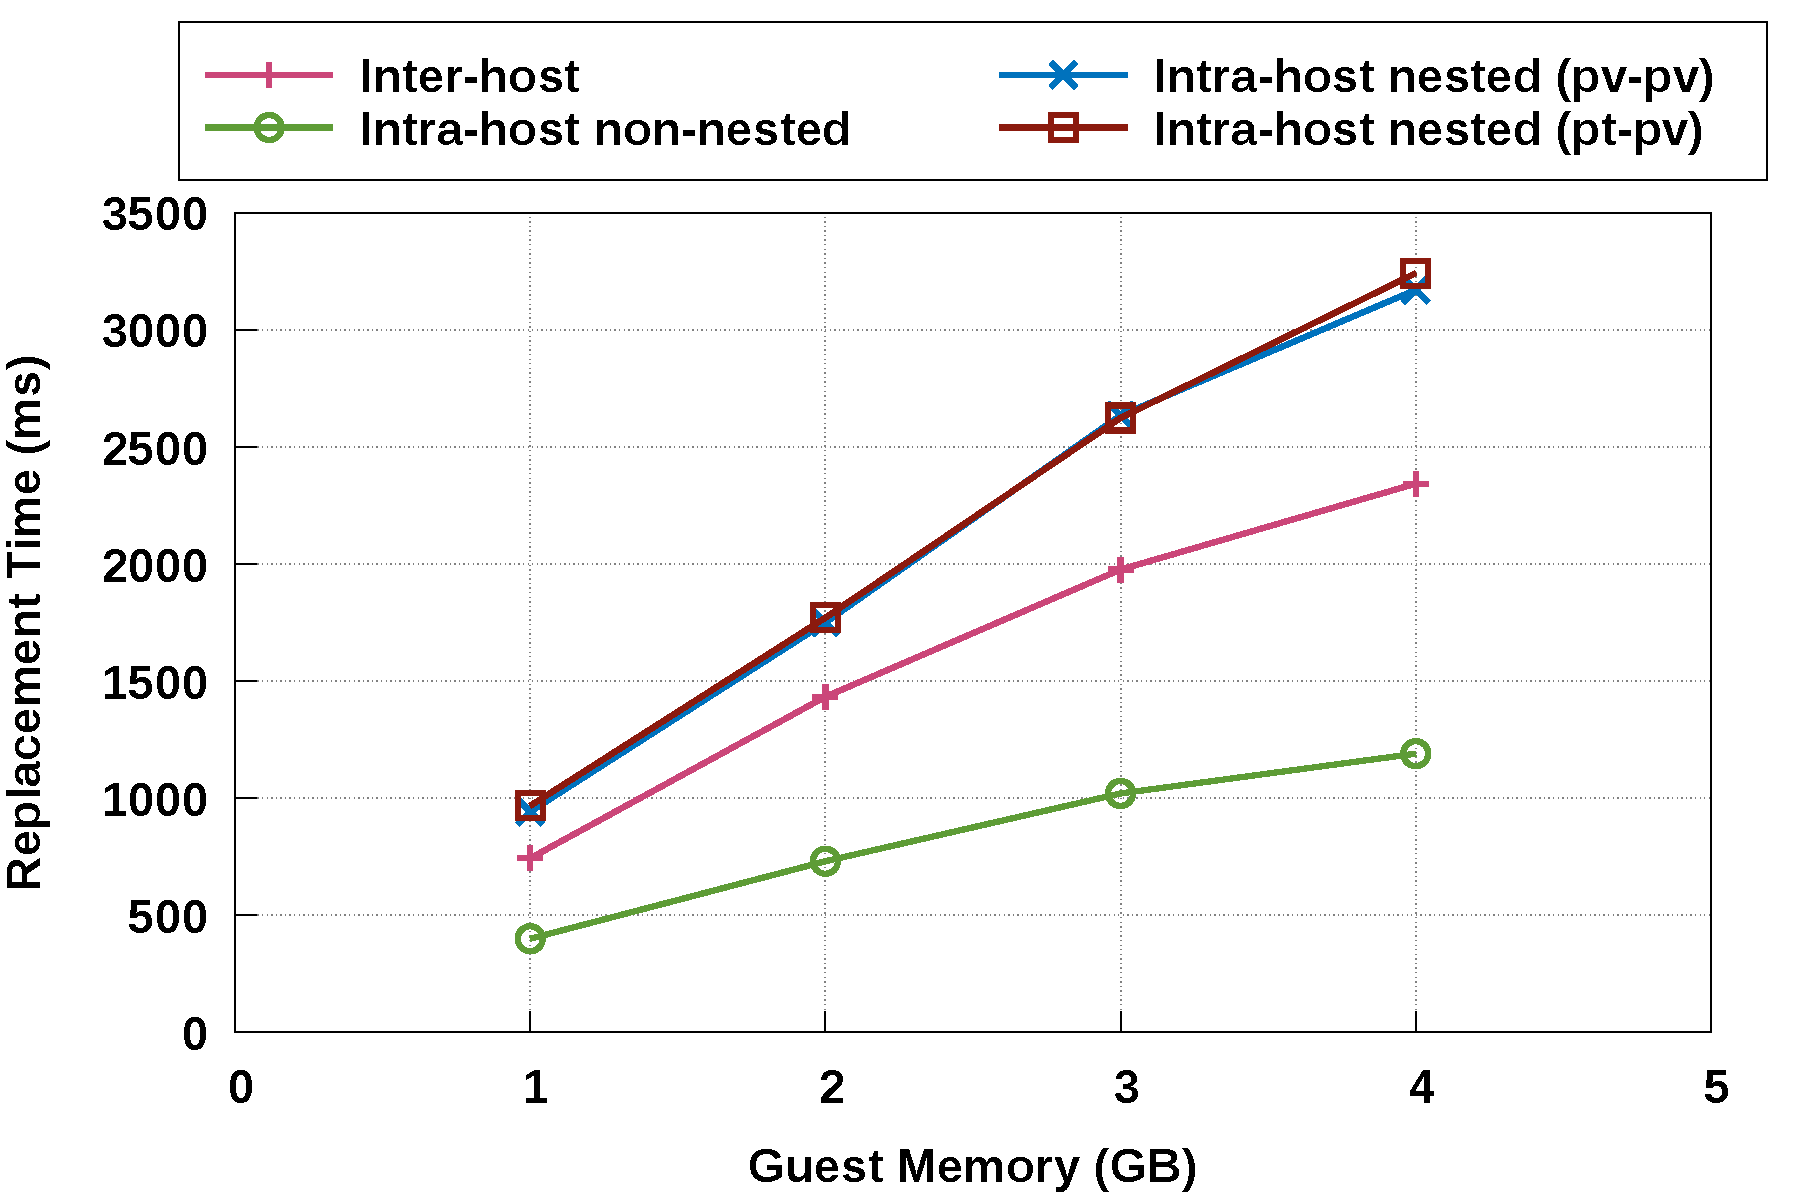
\includegraphics[width=.235\textwidth]{figures/busy_guest_migration.pdf}}
%	\caption{Replacement time comparison}
%	\label{fig:rt_motivation}
%\end{figure}

\subsection{Analysis of pre-copy performance for hypervisor replacement}
With the above optimizations to QEMU's default pre-copy live migration, 
we analyzed the total migration time, which also represents the time taken 
for hypervisor replacement operation.  We analyzed the following four configurations:
\begin{itemize}[leftmargin=0.15 in]
\parskip 0mm
\itemsep 0mm
\item {\bf Inter-host:} where a VM is migrated between two physical machines, as in Figure~\ref{fig:motivsetup}a. The source machine runs the stale hypervisor and the destination machine runs the new hypervisor.
\item {\bf Intra-host nested (pv-pv):} where the VM is migrated between two {\em co-located nested hypervisors}, as in Figure~\ref{fig:motivsetup}b. The source L1 runs the stale hypervisor and the destination L1 runs the new hypervisor. The network interfaces of both L1 hypervisors and their L2 VMs are configured as para-virtual {\em vhost-net} devices~\cite{vhost-net}.
\item {\bf Intra-host nested (pt-pv):} Same configuration as the above case, except that the both L1 hypervisors are configured to use pass-through network interfaces via virtual functions configured in the physical NIC.
\item {\bf Intra-host non-nested:} This is a baseline (and somewhat unrealistic) migration scenario where a single-level non-nested VM is migrated within the same host into another VM instance. This case helps us measure the intra-host live migration performance if there were no overheads due to nested virtualization and network interfaces (since source and destination QEMU processes communicate via the loopback device).
\end{itemize}
The experiments were conducted using machines having 10-core Intel-Xeon 2.2 GHz processors with 32GB memory 
and 40 Gbps Mellanox ConnectX-3 Pro network interface. 

Figure~\ref{fig:motiv}a plots the total migration time for an 
idle VM when the VM's memory size is increased 
from  1 GB to 4 GB. 
Figure~\ref{fig:motiv}b plots the total migration time for a busy VM
where the VM runs a write-intensive workload in the VM. Specifically, the 
write-intensive workload allocates a certain size of memory region and writes a few 
bytes to each allocated page at a controllable dirtying rate. 
The allocated memory size is 80\% of the VMs memory,  from 800 MB for a 1 GB VM to 3,200 MB for a 4 GB VM. 
The dirtying rate is set to 50,000 pages per second.

First we observe that in all the cases, as the VM size increases, 
the total migration time increases, because more memory pages must be transferred 
over a TCP connection for larger VMs. The migration times range from as low
as several hundred milliseconds for idle VMs to more than 3 seconds for 
busy write-intensive VMs. Since pre-copy retransmits dirtied pages from 
previous iterations, write-intensive VMs take longer to migrate.

The second surprising observation was that the {\em Inter-host} configuration  
for migrating a non-nested VM was faster than the {Intra-host}
configuration for migrating a nested VM. Replacing the para-virtual
{\em vhost-net} interface for the L1 hypervisor in the {\em Intra-host nested (pv-pv)} configuration with 
a pass-through interface in the {\em Intra-host nested (pt-pv)} configuration did not produce any noticeable
reduction in total migration time. 
%(However we did observe a reduction in 
%CPU utilization when pass-through I/O is used for the L1 hypervisor in the {\em pt-pv} case.)
To verify that this worse performance was caused by nesting overheads,
we carried out the {\em Intra-host non-nested} live migration described above. 
As expected, this fourth configuration performed better than the {\em Inter-host} 
configuration, confirming that nesting overheads indeed adversely affect 
intra-host VM migration.

Nevertheless, even in the ideal (though unrealistic) 
case represented by the {\em Intra-host non-nested} setting, 
traditional pre-copy migration takes between 0.4 seconds (for idle VM case)
to more than 1.19 seconds (for busy VM case) to migrate a single 4 GB busy VM. 
When multiple VMs must be relocated for hypervisor replacement, these 
times are bound to increase. We consider this performance unsatisfactory
for simply relocating VMs within the same host.

In summary, using intra-host pre-copy live migration for hypervisor 
replacement is expensive in terms of total migration time, network
overheads, and its affect on VM's performance. 
This motivates us to develop a much faster hypervisor replacement
technique based on memory remapping that does not involve copying of 
VM's memory pages within the same host. In the following sections,
we present our approach and show that our memory remapping-based
technique can achieve sub-10ms live hypervisor replacement times for VMs
and sub-second live OS replacement times for containers.

%During migration, the performance of VMs being migrated could be negatively impacted.  In addition, the large traffic generated during migration may impact other unrelated VMs sharing the same network infrastructure. These motivate us to seek a new technique for {\em fast} hypervisor/OS replacement. 

%-------------

%\para{Idle Case.} In \fref{fig:motivid}, we observe that, in the pre-copy live migration scenario, as the memory size of an idle VM increases, the total migration time increases accordingly. For example, the migration time increases from 346.2 ms for a 1 GB VM to 630.2 ms for a 4 GB VM for inter-host migration. Such an increase in total migration time is due to more memory transferred in pre-copy iteration rounds. 
%
%In contrast, we measured the migration time in the ``intra-host'' live migration scenario under nested virtualization.  We consider two typical configurations: (1) both L1 hypervisors and L2 VMs use the para-virtual driver; and (2) L1 hypervisors use  pass-through devices whereas L2 VMs use para-virtual driver. As shown in \fref{fig:motivid}, in comparison with the inter-host pre-copy scenario, we have the similar observation: as the memory size of the idle VM increases, the migration time also increases. Using either configuration 1 or 2, the ``intra-host'' case leads to higher total migration time compared to ``inter-host'' case. 
%%--- slightly higher when the memory size of the idle guest is 4 GB. 
%Though, with configuration 2, we do not observe much difference in terms of total migration time in comparison with configuration 1, we do observe lower CPU usage, as I/O pass-through eliminates the software overhead for L1.
%
%As hypervisor replacement occurs on the same host in our solution, we also measure the cost to migrate the guest on the same host. In \fref{fig:motivid}, the time spent in migrating a non-nested VM on the same host is still significantly high as the memory is still copied in multiple rounds. 
%
%%We also measure the total migration time to migrate a nested guest from one hypervisor to another on the same host. We consider two different configurations to measure migration of nested guest. In the first case, the hypervisor and the guest both use para-virtual driver to transmit the network packets. In the latter case, the hypervisor uses a pass-through device whereas the guest uses a para-virtual driver. 
%In \fref{fig:motivid}, the total migration time for the nested VM increases in both the cases compared to intra-host non-nested case due to the overhead induced by nested virtualization. In the figure, we see that these two configurations give almost the same performance. The difference in para-virtual/para-virtual(pv-pv) and pass-through/para-virtual(pt-pv) configuration is the CPU utilization on the host which is discussed in more detail in the design and evaluation sections.
%
%\para{Busy Case.} We run a write-intensive workload in the VM. More specifically, the write-intensive workload allocates a certain size of memory and dirties the memory by writing few bytes to the allocated memory at a controllable dirty rate. In the experiments, we vary the workload memory from 800 MB for a 1GB VM to 3200 MB for a 4 GB VM, which is 80\% of the memory and set the dirty rate to 50,000 pages per second. We migrate the VM after the given workload size is dirtied. 
%
%\fref{fig:motivbz} shows that, in all cases, the total migration time increases as the memory of the workload increases. It takes significant time to copy the working set memory over the network for inter-host migration (e.g., 2,342.6 ms for a 4 GB VM). 
%Again, the ``intra-host'' migration case without nested virtualization spends less time in migrating the VM, in comparison with the ``inter-host'' case.
%%a significant amount of memory copied on the same host. 
%The ``intra-host'' migration case with nested virtualization spends more time compared to the ``intra-host'' migration  without nested virtualization because of the nested virtualization overhead. 
%%Such overhead can be mitigated, if we use pass-through I/O devices for L1 hypervisor. 
%-------------


%The performance of the guest degrades considerably as the dirty page rate approaches the migration link bandwidth.
%The two factors that significantly affect the migration are page dirty rate and migration link bandwidth. The increase in dirty page rate increases the number of memory transfer rounds over the network. However, the downtime remains almost constant with varying dirty page rate as the number of pages transferred in the stop and copy phase is always less than 5000. In Fig. 2, a 2GB guest running a write-intensive application dirties memory at specified rate (pages / second). The migration link bandwidth is fixed to 1Gbps. We observe that the total migration time increases from abc to xyz as the page dirty rate increases. The downtime remains as low as 5ms. 

%If the migration link bandwidth increases, the total migration time and downtime decrease. A guest configured with 2GB memory and runs a memory intensive workload, zeusmp, a SPEC CPU2017 benchmark. The total migration time and downtime are measured as the migration link bandwidth is varied from 10Gbps to 40Gbps. From Fig. 3 and Fig. 4, the total migration time and downtime decrease as the migration link bandwidth increases. For a 10Gbps migration link bandwidth, the performance of the application running in the guest degrades due to high total migration time and downtime compared to 40Gbps migration link bandwidth.

%Setting the migration link bandwidth to a higher value improves the migration time but at the same time it generates huge network traffic. If the migration bandwidth is fixed to a lower value, the migration time increases and it affects the performance of the applications in the guest.
